% To je predloga za poročila o domačih nalogah pri predmetih, katerih
% nosilec je Blaž Zupan. Seveda lahko tudi dodaš kakšen nov, zanimiv
% in uporaben element, ki ga v tej predlogi (še) ni. Več o LaTeX-u izveš na
% spletu, na primer na http://tobi.oetiker.ch/lshort/lshort.pdf.
%
% To predlogo lahko spremeniš v PDF dokument s pomočjo programa
% pdflatex, ki je del standardne instalacije LaTeX programov.

\documentclass[a4paper,11pt]{article}
\usepackage{a4wide}
\usepackage{fullpage}
\usepackage[utf8x]{inputenc}
\usepackage[slovene]{babel}
\selectlanguage{slovene}
\usepackage[toc,page]{appendix}
\usepackage[pdftex]{graphicx} % za slike
\usepackage{setspace}
\usepackage{color}
\definecolor{light-gray}{gray}{0.95}
\usepackage{listings} % za vključevanje kode
\usepackage{hyperref}
\usepackage{float}
\renewcommand{\baselinestretch}{1.2} % za boljšo berljivost večji razmak
\renewcommand{\appendixpagename}{Priloge}

\lstset{ % nastavitve za izpis kode, sem lahko tudi kaj dodaš/spremeniš
language=Python,
basicstyle=\footnotesize,
basicstyle=\ttfamily\footnotesize\setstretch{1},
backgroundcolor=\color{light-gray},
}

\title{Inteligentni sistemi, 1. seminarska naloga}
\author{Matic Bernik in Robert Tovornik}
\date{\today}

\begin{document}

\maketitle

\section{Uvod}

Namen seminarske naloge je, da na podlagi podanih podaktov tekem NBA, 
zgradimo napovedni model, ga preverimo, ter z njim napovemo zmagovalca 
nove, prihodnje tekme, ter končno razliiko točk v koših med ekipama.

\section{Podatki}

V okviru seminarske naloge, so nam bili podani podatki tekem v NBA za pretekli 
 sezoni 2008/09 ter 2009/10. Ti se nahajajo v dveh datotekah: \\

\textendash  nba0809.txt 

\textendash  nba0910.txt

Skupaj obsegajo 2459 primerov, ter so opisani z 31 začetnimi atributi.
Med podatki ni mankajoči vrednosti (N/A).

\section{Pregled podatkov}

Ob zacetku, sva pregledala razporeditev podanih podatkov, s pomocjo orodja 
ORANGE (razvit na FRI), ter ugotovila, da so podatki razporejeni normalno, kar
 je zaželjeno ( razen podatkov o home in away team ).

\begin{figure}[H]
\begin{center}
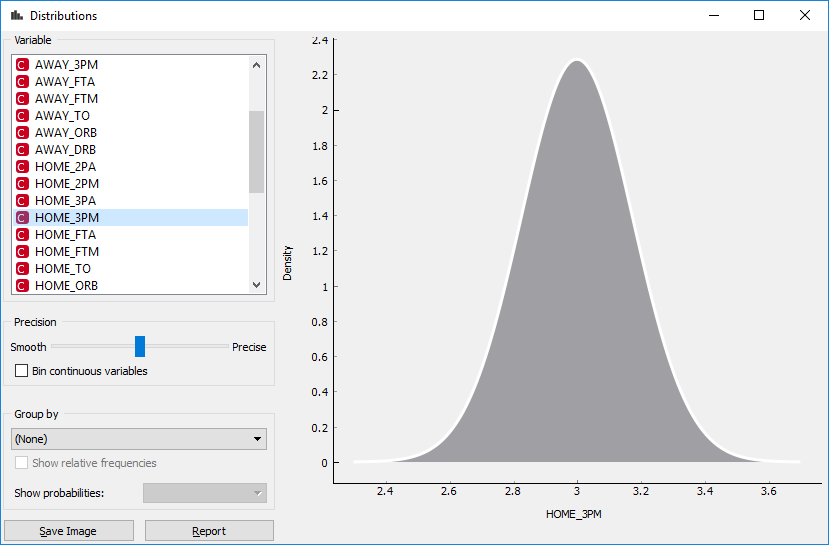
\includegraphics[scale=0.3]{OC_data_dist.png}
\caption{Prikaz razporeditve posamezni podatkov v orodju Orange (distributions).}
\label{slika1}
\end{center}
\end{figure} 

\section{Iskanje napovednih atributov in ustvarjanje novih}

Da bi lažje določila pomembnost atributov, ki določajo rezultat tekme, sva 
uporabila orodje Orange, za izračun teže informacije, oziroma ocene koliko 
določen atribut doprinese h končni napovedi. Le-te sva izračunala z ocenami atributov: 
 "Information gain", "Gain Ratio", "Gini" ter "ReliefF".

\begin{figure}[H]
\begin{center}
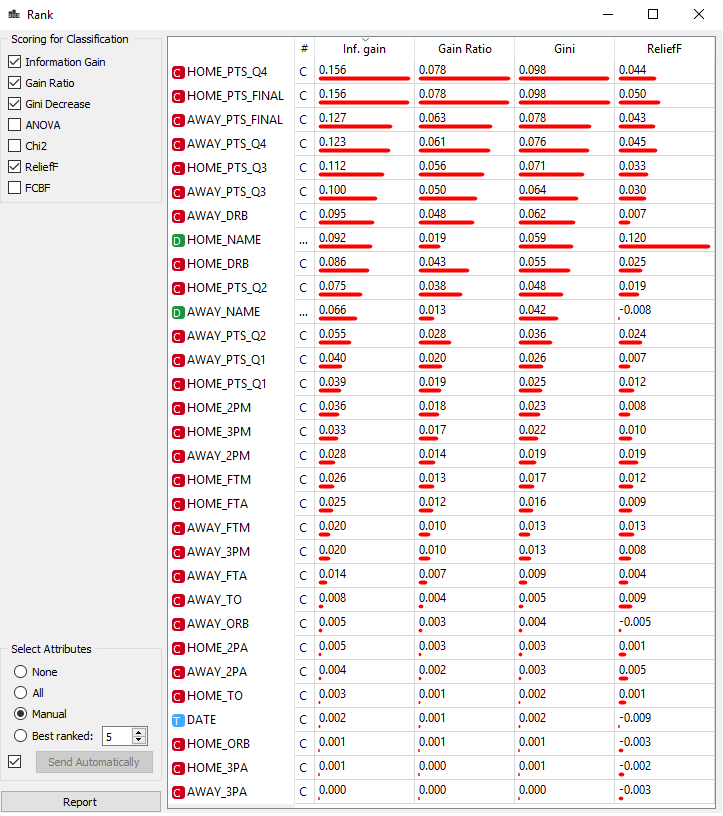
\includegraphics[scale=0.3]{OC_ranking_by_inf_gain.png}
\caption{Ocena teže oziroma informacijskega doprinosa atributov k napovedi.}
\label{slika2}
\end{center}
\end{figure} 

Presenetilo naju je, da poleg uspešnosti zadevanja koša, močno vplivajo tudi nekateri 
drugi atributi, med katerimi močno izstopa attribut "Defensive Rebounds". Po dodatnem testu, 
s funkcionalnostjo scatter plot, se je izkazalo, da močno nakazuje na končno število zadetih košev.

\begin{figure}[H]
\begin{center}
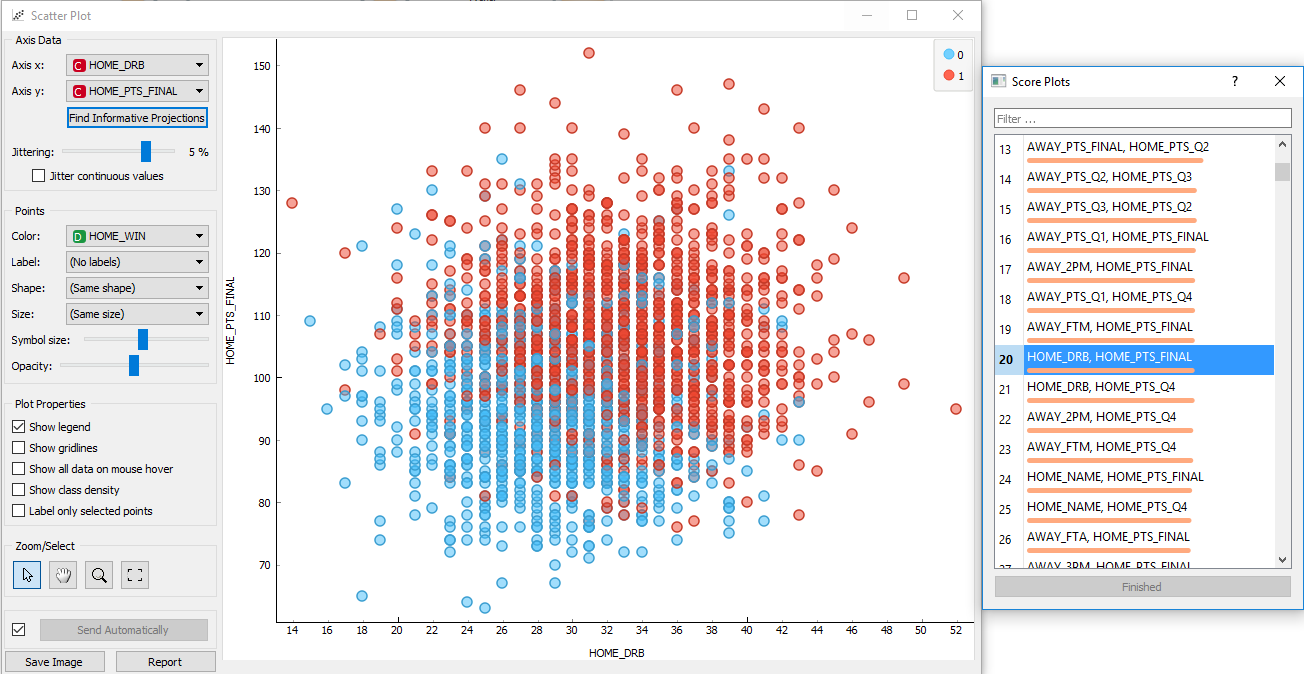
\includegraphics[scale=0.3]{OC_DRB_PTS-FINAL.png}
\caption{Scatter plot - relacija med "Defensive rebounds" in "Final points scored".}
\label{slika2.1}
\end{center}
\end{figure} 

Ko sva ocenila informacijske lastnosti atributov, sva se lotila iskanja možnosti združevanja 
in prepoznavanja sorodnosti atributov. Za to sva uporabila funkcionalnost orodja Orange,
HeatMap, ter hkrati clustering in opazila anomalijo, ki jo povzroča datum, ki tekme unikatno
 določa. Zato sva le-tega odstranila iz učnih podatkov, ter ponovno zagnala prepoznavanje.\\


\begin{figure}[H]
    \centering
    \begin{minipage}{0.5\textwidth}
        \centering
        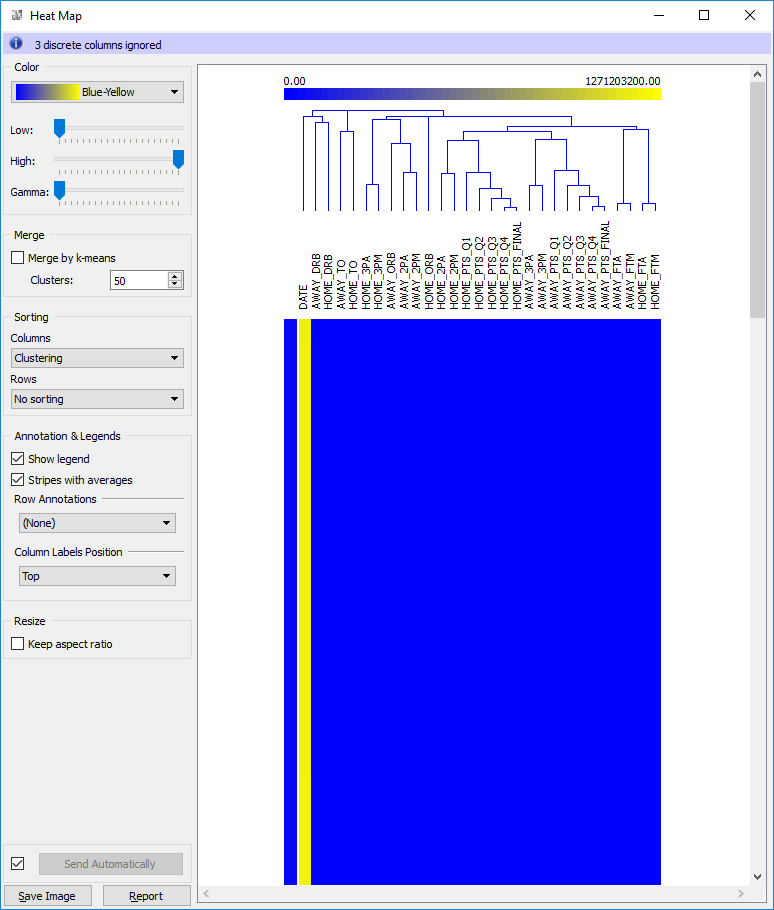
\includegraphics[width=0.9\textwidth]{OC_attrib-cluster.png}
        \caption{Heatmap z datumom}
        \label{slika3.1}
    \end{minipage}\hfill
    \begin{minipage}{0.5\textwidth}
        \centering
        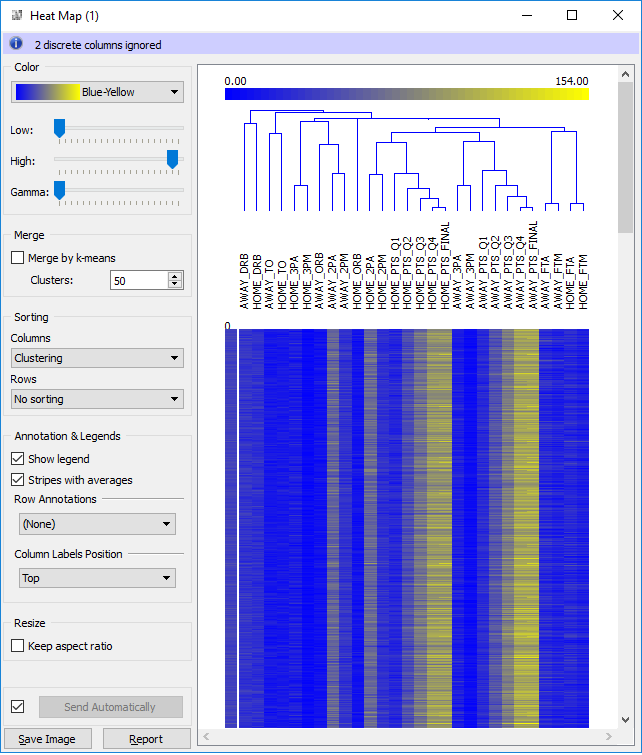
\includegraphics[width=0.9\textwidth]{OC_attrib-cluster-no_date.png}
        \caption{Heatmap, datum odstranjen}
        \label{slika3.2}
    \end{minipage}
\end{figure}

Nato sva prišela s postopko združevanja atributov. Zaradi boljše verjetnosti 
kasnejšega napovedovanja, sva se odločila za pristop statističnega napovedovanja 
pričakovane vrednosti posameznega atributa, za vsako ekipo posebej, na podlagi 
vrednosti atributov v preteklosti odigranih tekem. Tako sva združila npr. za posamezne 
kategorije metov število metov in število uspšeni v odstotek uspešnih metov, na podlagi 
števila prostih metov izračunala število prekrškov, ki jih je storila nasprotna ekipa
 (delitev z dva, kot je ponavadi število prostih metov za prekršek), ostale preproste atribute 
pa sva ocenila po pričakovani vrednosti.

\section{Metode}

\subsection{Testiranje}

Da lahko ugotovimo natančnost in uspešnost naših atributov oziroma 
napovedni modelov, je potrebno testiranje. Osnovna metoda testiranja 
je delitev vseh podanih primerov na učno ter testno množico. Da 
zagotovimo optimalno oceno, morata ti dve množici biti povsem ločeni 
oziroma neodvisni. 

Ker je narava podane naloge takšna, da je pogoj, da gradimo naše učne 
modele zgolj na podlagi podatkov tekem ki so se zgodile predohdno, je 
sicer izjemno učinkovit način k-kratnega prečnega preverjanja odpadel. 
Odločila sva, da je pametneje in nekako edino možno, da uporabimo delitev 
po razmerju 70 - 30 procentov, kjer so vsi primeri najprej primerno razvrščeni
 po datumu padajoče. Tako 70 procentov hkrati predstavlja prvih 70 procentov 
vseh primerov in 30 procentov zadnjih 30 procentov vseh primerov. Prav tako 
ni bil izveden običajen korak premešanja podatkov, prav z razlogom ohranitve 
časovnega zaporedja.

Da bi zagotovila primernost delitve, sva jo tudi testirala z uporabo večinskega 
klasifikatorja nad učno ter nad testno množico. Rezultati so bili zadovoljivo blizu.

\begin{table}[H]
\caption{Primerjava večinskega klasifikatorja nad splošno, učno ter testno množico.}
\label{tab1}
\begin{center}
\begin{tabular}{llp{3cm}}
\hline
Splošen klasifikator & Test nad učno množico & Test nad testno množico \\
\hline
0.601302 & 0.610691 & 0.579946 \\
\hline
\end{tabular}
\end{center}
\end{table}

\subsection{Klasifikacija}

Prvi korak pri klasifikaciji je bil, da sva iz podatkov odstranila atribut 
"final score differencial", ki je napovedni objekt regresije.

Da bi lahko ocenila, ali klasifikacija deluje primerno, ter ali so atributi 
primerno ustvajeni, sva najprej klasificirala po metodi prevladujočega razreda 
"Majority classifier". Rezultate tega, sva privzela kot spodnjo mejo, za ovržbo 
metod, ki bi dosegle rezultate pod le-to.

Sledila je klasifikacija po sledečih metodah, z doseženimi pripadajočimi 
rezultati. Ocenjevala sva natančnost klasfikacije, pripadajočo oceno Brier, 
obcutljivost, specificnost, ter izrisala ROC krivujlo.

\begin{table}[H]
\caption{Metode klasifikacije ter pripadajoča uspešnost.}
\label{tab1}
\begin{center}
\begin{tabular}{lllllp{3cm}}
\hline
Metoda & Natančnost & Brier score & Sensitivity & Specificity & Ploščina pod krivuljo ROC\\
\hline
Majority & 0.601302 & - & - & - & - \\
\hline
DecTree & 0.615176 & 0.524994 & 0.710280 & 0.483871 & 0.6121 \\
kNN & 0.649051 & 0.447209 & 0.803738 & 0.435484 & 0.6753 \\
rPart & 0.650407 & 0.456028 & 0.747664 & 0.516129 & 0.6685 \\
RandForest & 0.653117 & 0.443033 & 0.880841 & 0.338710 & 0.6728 \\
SVM & 0.658537 & - & 0.871495 & 0.364516 & 0.6728 \\
NaiveBayes & 0.665312 & 0.540539 & 0.775701 & 0.512903 & 0.7065 \\
\hline
Q2	-  spremembe \\
\hline
DecTree & 0.612466 & 0.551575 & 0.764019 & 0.403226 & 0.6226 \\
RandForest & 0.639566 & 0.446379 & 0.873832 & 0.316129 & 0.6655 \\
kNN & 0.644986 & 0.445738 & 0.801402 & 0.429032 & 0.6671 \\
SVM & 0.651762 & - & 0.866822 & 0.354839 & - \\
NaiveBayes & 0.658537 & 0.540635 & 0.768692 & 0.506452 & 0.7059 \\
\hline
Q3	-  spremembe \\
\hline
DecTree & 0.631821 & 0.525576 & 0.696262 & 0.500000 & 0.6026 \\
RandForest & 0.638211 & 0.443600 & 0.862150 & 0.329032 & 0.6703 \\
kNN & 0.650407 & 0.445488 & 0.813084 & 0.425806 & 0.6781 \\
SVM & 0.651762 & - & 0.864486 & 0.358065 & - \\
NaiveBayes & 0.663957 & 0.540805 & 0.773364 & 0.512903 & 0.7057 \\
\hline
\end{tabular}
\end{center}
\end{table}

Ker NaiveBayes predpostavlja neodvisnost atributov, sva se ga odlocila zanemarit.
"S hitrim premislekom lahko ugotovimo da sta že met za 2 in 3 pike povezana. Če nekdo 
nebi znal metati za 2 pike in zadeti, bi posledično tudi za 3 pike metal slabo."

Zato sva izbrala kot najboljšo klasifikacijsko metodo kar SVM.

\begin{figure}[H]
\begin{center}
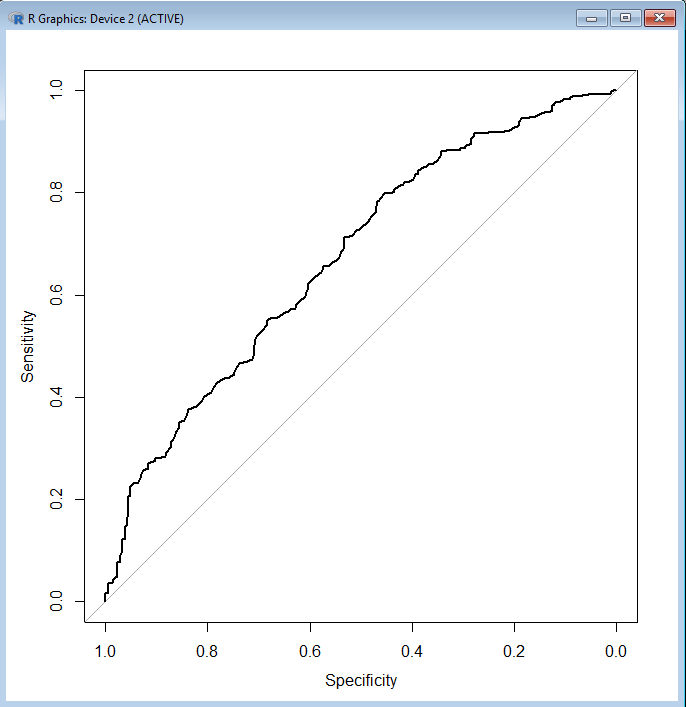
\includegraphics[scale=0.5]{9_SVM_roc.png}
\caption{SVM pripadajoča ROC krivulja .}
\label{slika4}
\end{center}
\end{figure} 


\subsection{Regresija}

Pri regresiji pa je bil prvi korak ravno obraten kot pri klasifikaciji, najprej
sva odstranila atribut "Home win", saj je napovedni objekt klasifikacije.

Pri ocenjevanju regresije, sva uporabila vrsto ocen, na različnih modelih: 
MAE, RMAE, MSE ter RMSE, kot je razvidno iz sledeče tabele


\begin{table}[H]
\caption{Metode regresije ter pripadajoča uspešnost.}
\label{tab1}
\begin{center}
\begin{tabular}{llllp{3cm}}
\hline
Metoda & MAE & RMAE & MSE & RMSE\\
\hline
RegTree & 10.325824 & 0.964280 & 167.115254 & 0.939377 \\
LinReg & 10.372827 & 0.968670 & 167.086603 & 0.939216 \\
NeuralNet & 10.168043 & 0.949546 & 166.457396 & 0.935679 \\
SVM & 10.003695 & 0.934198 & 156.683559 & 0.880739 \\
RandForests & 9.905421 & 0.925021 & 155.271914 & 0.872804 \\
\hline
Q2	- sprememba \\
\hline
NeuralNet & 10.310324 & 0.962833 & 168.892140 & 0.949365 \\
LinReg & 10.372770 & 0.968664 & 167.104486 & 0.939316 \\
SVM & 10.041344 & 0.937714 & 158.245159 & 0.889517 \\
RandForests & 9.802771 & 0.915435 & 153.416885 & 0.862377 \\
\hline
Q3	- sprememba \\
\hline
LinReg & 10.398817 & 0.971097 & 167.889116 & 0.943727 \\
NeuralNet & 10.070732 & 0.940458 & 160.490729 & 0.902140 \\
SVM & 10.038235 & 0.937424 & 158.002436 & 0.888153 \\
RandForests & 9.953541 & 0.929515 & 157.265529 & 0.884010 \\
\hline
\end{tabular}
\end{center}
\end{table}

Kot se izkaže, najbolje nad podanimi podatki deluje model "Random 
Forests". 


\section{Rezultati}



\end{document}
